\documentclass[border=10pt]{standalone}

\usepackage{tikz}
\usepackage{tikzsymbols}
\usetikzlibrary{calc,patterns,shapes.geometric}

\def\centerarc[#1](#2)(#3:#4:#5){\draw[#1] ($(#2)+({#5*cos(#3)},{#5*sin(#3)})$) arc (#3:#4:#5);}

\begin{document}
	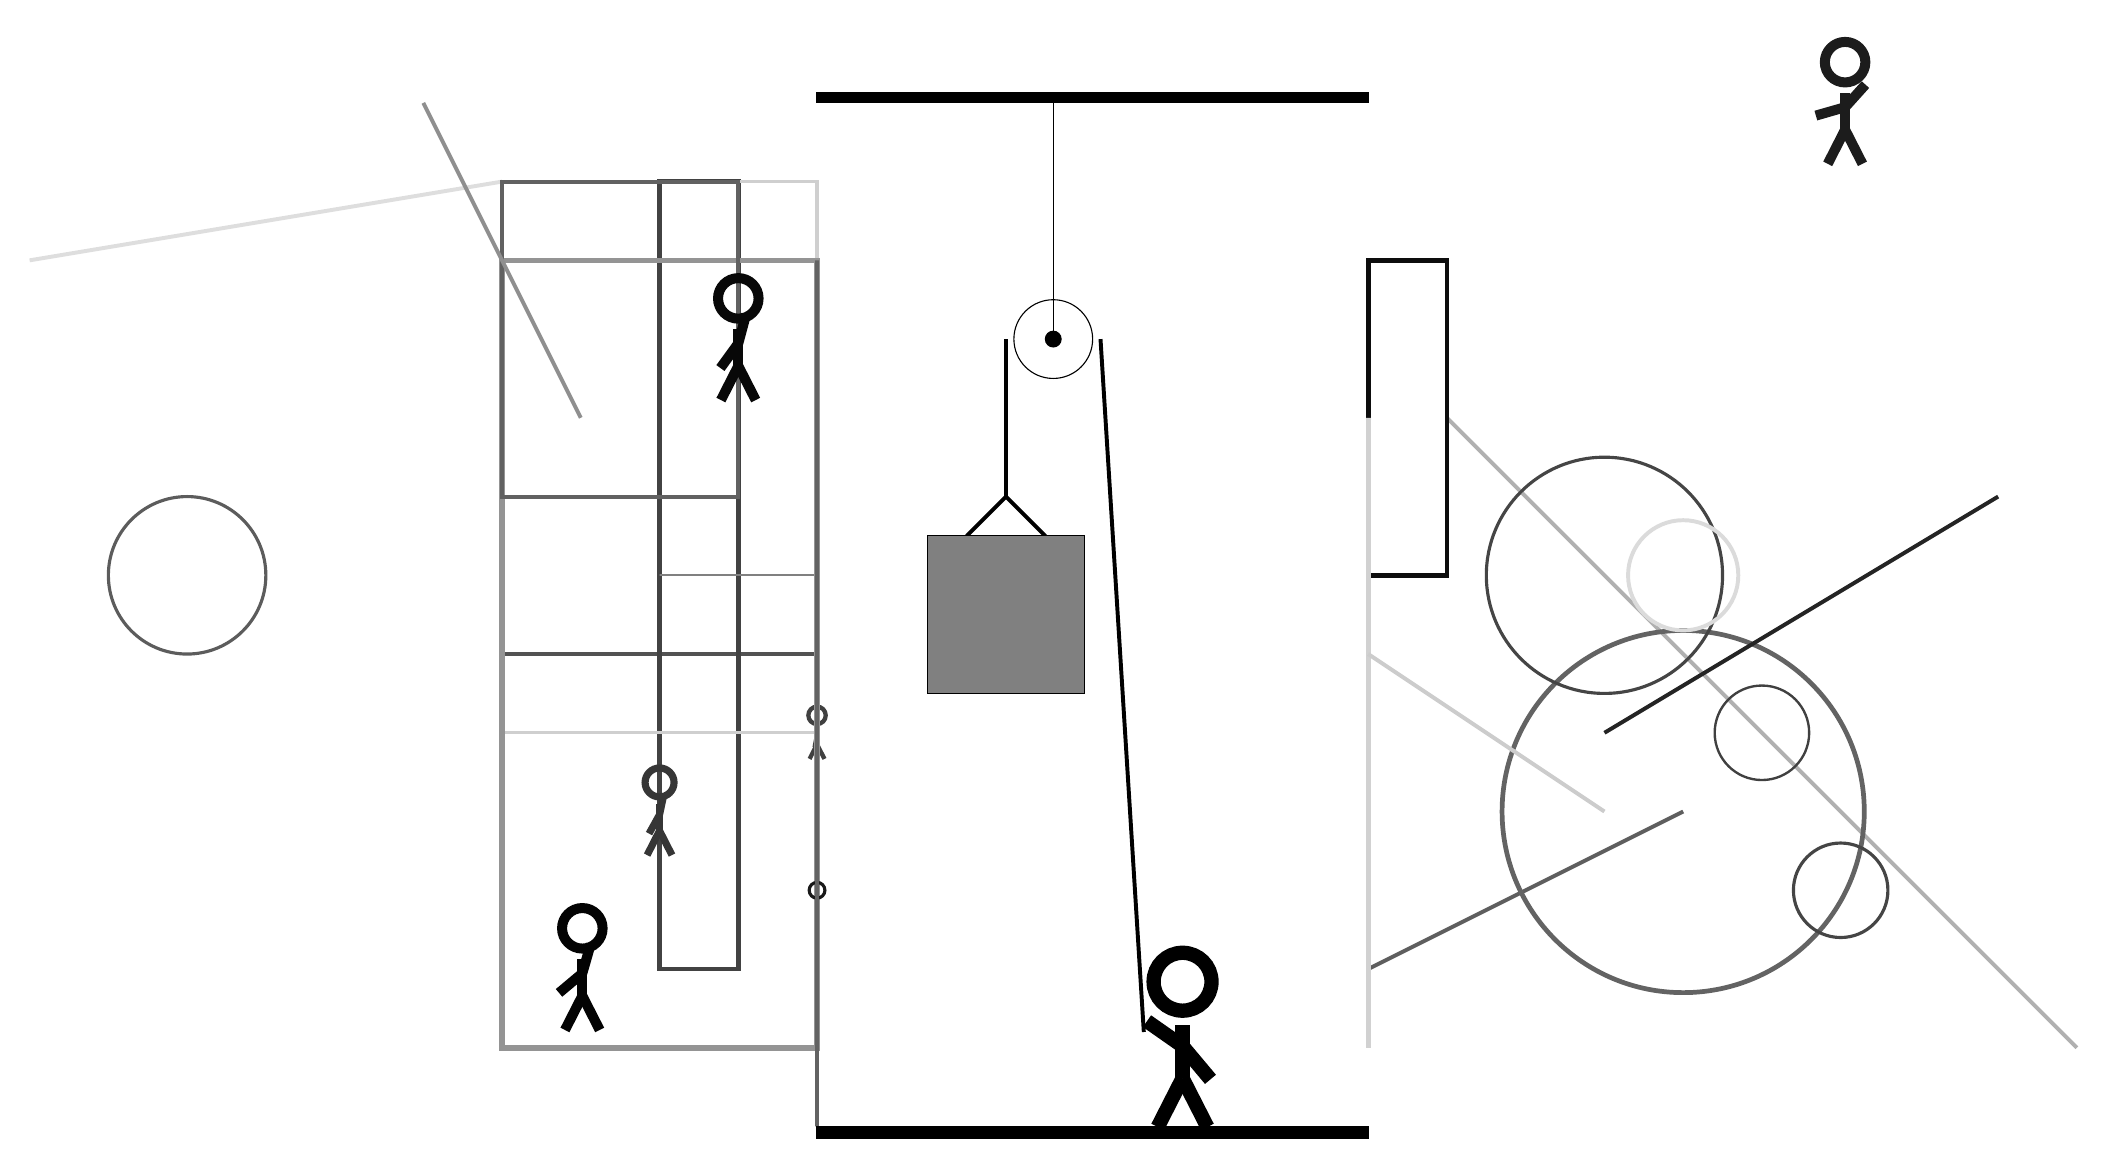
\begin{tikzpicture}
		%%%%% START %%%%%
		
		\draw[fill=black] (-2, 10) rectangle (5, 10.125);
		
		\draw (1, 7) circle (0.5);
		\draw[fill=black] (1, 7) circle (0.1);
		\draw (1, 10) -- (1, 7);
		
		\draw[line width=0.5mm] (-0.1, 4.5) -- (0.4, 5.0) -- (0.9, 4.5);
		\draw[fill=black!50] (-0.6, 4.5) rectangle (1.4, 2.5);
		
		\draw[line width=0.5mm] (0.4, 7) -- (0.4, 5.0);
		\centerarc[line width=0.5mm](1, 7)(0:180:0.6);
		\draw[line width=0.5mm](1.6, 7) -- (2.15, -1.8);
		
		\draw [line width=0.4mm, color=black!64](-10, 4) circle (1.0);
		
		\draw[line width=0.5mm, color=black!31](6, 6) -- (14, -2);
		\node[line width=0.5mm, color=black!75] at (-2, 2) {\Strichmaxerl[3][79][88]};
		\draw[line width=0.5mm, color=black!13](-6, 9) -- (-12, 8);
		\draw[line width=0.5mm, color=black!63](5, -1) -- (9, 1);
		\draw[line width=0.6mm, color=black!95] (5, 8) rectangle (6, 4);
		
		\draw[line width=0.4mm, color=black!68] (-2, 2) rectangle (-6, 3);
		
		\draw[line width=0.6mm, color=black!74] (-3, -1) rectangle (-4, 9);
		\draw[line width=0.4mm, color=black!19] (-2, 2) rectangle (-6, 9);
		\draw [line width=0.6mm, color=black!61](9, 1) circle (2.3);
		\draw[line width=0.3mm, color=black!50] (-2, 4) rectangle (-4, 4);
		
		\draw [line width=0.4mm, color=black!73](8, 4) circle (1.5);
		\node[line width=0.4mm, color=black!89] at (11, 10) {\Strichmaxerl[7][16][48]};
		
		\node[line width=0.3mm, color=black!79] at (-4, 1) {\Strichmaxerl[5][61][78]};
		\draw [line width=0.5mm, color=black!14](9, 4) circle (0.7);
		\node[line width=0.4mm, color=black!99] at (-5, -1) {\Strichmaxerl[7][40][74]};
		\draw[line width=0.7mm, color=black!42] (-2, 8) rectangle (-6, -2);
		
		\draw [line width=0.4mm, color=black!90](-2, 0) circle (0.1);
		\draw[line width=0.6mm, color=black!18] (5, 6) rectangle (5, -2);
		
		\draw[line width=0.5mm, color=black!62] (-3, 5) rectangle (-6, 9);
		\draw[line width=0.5mm, color=black!44](-5, 6) -- (-7, 10);
		
		\draw [line width=0.4mm, color=black!73](11, 0) circle (0.6);
		
		\draw[line width=0.3mm, color=black!62] (-2, 10) rectangle (-2, 10);
		\draw[line width=0.5mm, color=black!20](8, 1) -- (5, 3);
		\draw [line width=0.3mm, color=black!75](10, 2) circle (0.6);
		
		\draw[line width=0.5mm, color=black!86](8, 2) -- (13, 5);
		\node[line width=0.4mm, color=black!97] at (-3, 7) {\Strichmaxerl[7][54][75]};
		\draw[line width=0.4mm, color=black!61] (-2, 8) rectangle (-2, -3);
		
		\node at (2.6, -1.9) {\Strichmaxerl[10][-35][-50]};
		
		\draw[fill=black] (-2, -3) rectangle (5, -3.15);
		
		%%%%% END %%%%%
	\end{tikzpicture}
\end{document}